%%% DOCUMENT SETUP %%%
\documentclass[11pt,a4paper,onecolumn]{article}
\usepackage[english]{babel}

%%% LAYOUT %%%
\usepackage{fullpage}
\usepackage[parfill]{parskip}
\usepackage{multicol}
\usepackage{footnote}

%%% GRAPHICS %%%
\usepackage{graphics}
\usepackage{color}
\usepackage{graphics}
\usepackage{rotating}
\usepackage{subfig}
\usepackage{amsmath}
\usepackage{amssymb}
\usepackage{amscd}
\usepackage{xfrac}
\usepackage{float}
\usepackage{dsfont}
\usepackage{mathtools}
\usepackage{wrapfig}

%%% FONT %%%
\usepackage{ifxetex}
\ifxetex
  \usepackage{fontspec}
    \setmainfont{Linux Libertine O}
  \usepackage{xunicode}
  \usepackage{microtype}
\else
  \usepackage[T1]{fontenc}
  \usepackage[latin1]{inputenc}
  \usepackage{times}
  \usepackage{microtype}
\fi

%%% Coding %%%
\usepackage{listings}
\usepackage{pseudocode}

%%% TITLE PAGE %%%
\author{Jeroen Hofman (10194754)  \\[15pt] University of Amsterdam (\textsc{UvA})}

\title{Computational Biology\\
  Lab exercises 
		}

\begin{document}
\maketitle
\captionsetup{width=0.8\textwidth}
\lstset{language=Mathematica,breaklines=true,backgroundcolor=\color{white},frame=single,showspaces=false,basicstyle=\footnotesize}
\thispagestyle{empty}
\graphicspath{{/home/jhofman/Desktop/CompBio/lab1/}{/home/jhofman/Desktop/CompBio/lab2/}{/home/jhofman/Desktop/CompBio/lab3/}{/home/jhofman/Desktop/CompBio/lab4/}{/home/jhofman/Desktop/CompBio/lab5/}}


%%% TABLE OF CONTENTS %%%
\newpage
\tableofcontents
\newpage

\section{Lab1: Introduction}
\subsection{Exercise 1: Bacteria growth}

We have the following differential equation:

\begin{equation*}
  \frac{dx}{dt} = C x
\end{equation*}

which has a solution given by:

\begin{lstlisting}[mathescape]
solx = DSolve[{x'[t]==C x[t],x[0]==10},x[t],t]
\end{lstlisting}
\begin{lstlisting}[mathescape]
{{x[t] -> 10 E^(C t)}}
\end{lstlisting}

we can now use this solution to solve for $C$ given the initial conditions:

\begin{lstlisting}[mathescape]
solC = Solve[(2x[t]/.solx/.t->0)==(x[t]/.solx/.t->20),C]
\end{lstlisting}
\begin{lstlisting}[mathescape]
{{C -> Log[2]/20}}
\end{lstlisting}

Now if we want to know when the density takes 8 or 10 times the original value, we check when the solution found above is 8 or 10 times the initial solution with $t = 0$:

\begin{lstlisting}[mathescape]
(*Solve when value has reached x times start value*)
Solve[(x[t]/.solx/.solC)==(8 x[t]/.solx/.solC/.t->0),t]
Solve[(x[t]/.solx/.solC)==(10 x[t]/.solx/.solC/.t->0),t]//N
\end{lstlisting}
\begin{lstlisting}[mathescape]
{{t -> 60}}
{{t -> 66.4386}}
\end{lstlisting}

We find that the value is 8 or 10 times the original value when t = 60 or t = 66.4386 respectively.

\subsection{Exercise 2: Growth Model}

Given the data set, we can fit both exponential and linear curves using \texttt{FindFit}. We obtain the following results:

\begin{lstlisting}[mathescape]
data = {{0.5,1.27},{0.6,6.58},{0.7,7.00},{0.8,8.83},{0.9,8.66},
{1.0,5.53},{1.1,9.33},{1.2,14.57},{1.3,8.51},{1.4,17.61},
{1.5,12.94},{1.6,18.45},{1.7,19.85},{1.8,25.03},{1.9,28.14},
{2.0,28.31},{2.1,33.41},{2.2,41.43},{2.3,40.87},{2.4,56.71},
{2.5,59.32}};
expFit = FindFit[data,a + b Exp[c x],{a,b,c},x]
linFit = FindFit[data,a + b x,{a,b},x]
Show[ListPlot[data],Plot[a + b Exp[c x]/.expFit,{x,0,2.5}],Plot[a + b x/.linFit,{x,0,2.5}]]
\end{lstlisting}
\begin{lstlisting}[mathescape]
{a -> 1.48353, b -> 1.70259, c -> 1.41534}
{a -> -15.9278, b -> 24.9788}
\end{lstlisting}

\begin{figure}[H]
  \centering
  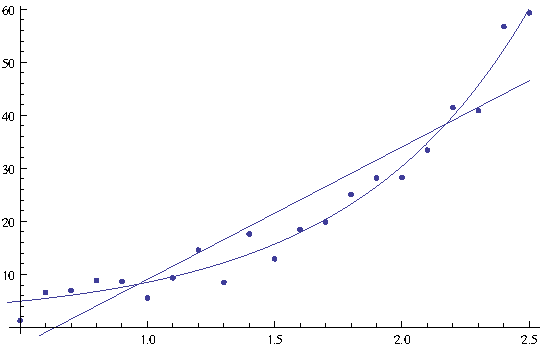
\includegraphics[width=0.48\textwidth]{lab1_ex_gr1.pdf}
\end{figure}

The parameters are given above after the code, and are the best fits for the functions $a + be^{cx}$ and $a + bx$. From the figure above it is clear that the exponential fit is a much better fit (judging by eye). This can be made more precise by doing an ANOVA analysis on the outcome of the fit, however this is not the point of the exercise.

\subsection{Exercise 3: Population Dynamics}

Starting from the following differential equation:

\begin{equation*}
  \frac{dx}{dt} = f(x) = \frac{2 x^m}{1 + x^4}
\end{equation*}

we first sketch $f(x)$ in the figure below, both for m = 1 (red) and m = 2 (blue) and then solve $f(x) = 0$ to find the stationary points, the stability of these stationary points is evaluated by looking at the sign of $f'(x)$ at those points, this is performed for $m = 1$ and $m = 2$ in the code below:

\begin{lstlisting}[mathescape]
f[x_] = 2 x^m/(1 + x^4)-x;
Show[Plot[f[x]/.{m->1},{x,0,1.5},PlotRange->All,PlotStyle->Red],Plot[f[x]/.{m->2},{x,0,1.5},PlotRange->All,PlotStyle->Blue]]
roots = Solve[(f[x]/.{m->1})==0,x,Reals]
f'[x]/.m->1/.roots
roots = NSolve[(f[x]/.{m->2})==0,x,Reals]
f'[x]/.m->2/.roots
\end{lstlisting}
\begin{lstlisting}[mathescape]
{{x -> -1}, {x -> 0}, {x -> 1}}
{-2, 1, -2}
{{x -> 0.}, {x -> 0.543689}, {x -> 1.}}
{-1., 0.678574, -1.}
\end{lstlisting}

\begin{figure}[H]
  \centering
  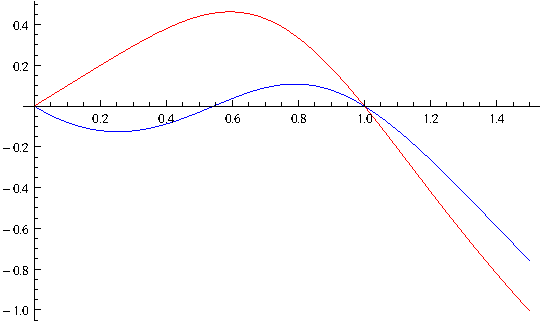
\includegraphics[width=0.48\textwidth]{lab1_ex_gr2.pdf}
\end{figure}

From the output we find stationary points at $x = 0$ (unstable) and $x = 1$ (stable) for $m = 1$ and $x = 0$ (stable), $x = 0.543689$ (unstable) and $x = 1$ (stable) for $m = 2$.

The behavior for small initial conditions ($x(0) = 0.01$) and large initial conditions ($x(0) = 100$) are given by the following code and figure:

\begin{lstlisting}[mathescape]
fitSmall = DSolve[{{x'[t]==((2 x[t]^m/(1 + x[t]^4))-x[t])/.m->1},{x[0]==0.01}},x[t],t];
fitLarge= DSolve[{{x'[t]==((2 x[t]^m/(1 + x[t]^4))-x[t])/.m->1},{x[0]==100}},x[t],t];
fitSmall2 = NDSolve[{{x'[t]==((2 x[t]^m/(1 + x[t]^4))-x[t])/.m->2.},{x[0]==0.01}},x[t],{t,0,10}]
fitLarge2= NDSolve[{{x'[t]==((2 x[t]^m/(1 + x[t]^4))-x[t])/.m->2.},{x[0]==100}},x[t],{t,0,10}];
Show[Plot[x[t]/.Flatten[fitSmall][[1]],{t,0,10},PlotRange->{{0,10},{0,10}}],Plot[x[t]/.Flatten[fitLarge][[1]],{t,0,10}],
Plot[Evaluate[x[t]/.fitSmall2],{t,0,2},PlotStyle->Red],Plot[Evaluate[x[t]/.fitLarge2],{t,0,10},PlotStyle->Red]]
\end{lstlisting}

\begin{figure}[H]
  \centering
  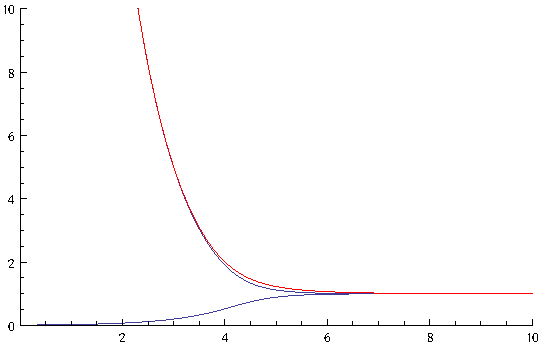
\includegraphics[width=0.48\textwidth]{lab1_ex_gr3.pdf}  
\end{figure}

In the figure the blue lines are the lines corresponding to $m = 1$ and we see that with both initial conditions the solution converges to 1, which is a stable point as we found above. For the case of $m = 2$ (the red lines) the dynamics with the large initial condition converge to 1, however the other solution converges to 0 (not clearly visible), which are indeed both stable points, so this analysis reconfirms our stable points.

\subsection{Exercise 4: Finite Difference Equation}

We have the finite difference equation:

\begin{equation*}
  \phi_{t+1} = f(\phi) = 0.5 + \alpha \text{sin}(2\pi phi_{t})
\end{equation*}

where we can find the steady states by solving $\phi_{t+1} = \phi_{t}$ for different values of $\alpha \leq 0.5$. The solution is always $\phi = 0.5$ for various values of $\alpha$,as the code below shows:

\begin{lstlisting}[mathescape]
f[$\phi$_] = 0.5 + $\alpha$ Sin[2\[Pi] $\phi$];
sola=FindRoot[(f[$\phi$]/.$\alpha$->0.0)-$\phi$,{$\phi$,0.5}]
sola=FindRoot[(f[$\phi$]/.$\alpha$->0.25)-$\phi$,{$\phi$,0.5}]
solb=FindRoot[(f[$\phi$]/.$\alpha$->0.5)-$\phi$,{$\phi$,0.5}]
\end{lstlisting}
\begin{lstlisting}[mathescape]
{$\phi$ -> 0.5}
{$\phi$ -> 0.5}
{$\phi$ -> 0.5}
\end{lstlisting}

The stability can be analyzed by calculating the absolute value of the derivative of the function in the steady state:

\begin{equation*}
  |f'(\phi)| = |2\pi \alpha \text{cos}(2\pi 0.5)| = |-2\pi \alpha| = 2\pi \alpha
\end{equation*}

If $|f'(\phi)| < 1$ the steady state is stable, hence when $\alpha < \sfrac{1}{2\pi} \approx 0.16$ the solution will be stable, at $\alpha = \sfrac{1}{2\pi}$ the steady state is unknown in terms of stability and when $\alpha > \sfrac{1}{2\pi}$ the solution is non-stable.

Finally we sketch $f(\phi)$ as a function of $\phi_t$ for $\alpha = 0.25$ (the dashed line). We find a maximum at 0.25, a minimum at 0.75 and an inflection point at 0.5. We also plot $\phi_t$ (solid thin line) and $f(f(\phi))$ (thick line) and look for a point where $f(f(\phi)) = \phi$ but $f(\phi) \neq \phi$. From the figure we see that the only possibilities are 0.25 and 0.75 (for 0.5 the second condition is not met). And indeed, if we solve this we see that 0.25 is indeed a stable period-2 orbit.

\begin{lstlisting}[mathescape]
Show[Plot[$\phi$,{$\phi$,0,1}],Plot[f[f[$\phi$]]/.$\alpha$->0.25,{$\phi$,0,1},PlotStyle->Thick],Plot[(f[$\phi$]/.$\alpha$->0.25),{$\phi$,0,1},PlotStyle->Dashed]]
FindRoot[$\phi$ == (f[f[$\phi$]]/.$\alpha$->0.25),{$\phi$,0.2}]
\end{lstlisting}
\begin{lstlisting}[mathescape]
{$\phi$ -> 0.25}
\end{lstlisting}

\begin{figure}[H]
  \centering
  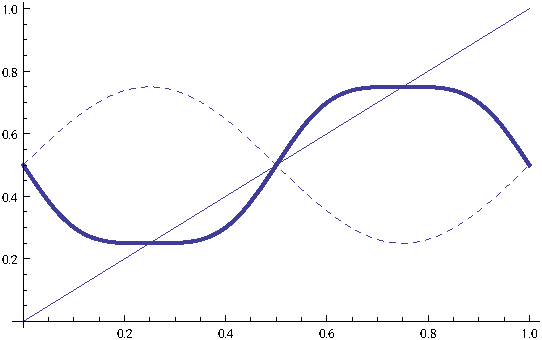
\includegraphics[width=0.48\textwidth]{lab1_ex_gr4.pdf}  
\end{figure}

\subsection{Exercise 5: The Game of Life}

We used the Python code provided on Blackboard and altered it slightly to meet the conditions given in the exercise:

\lstinputlisting[language=Python]{/home/jhofman/Desktop/CompBio/lab1/GoL.py}

Since the code is working correctly there is not much more to say about this exercise. I played around a bit with different initial conditions and rules.


\newpage

\section{Lab2: Sequence Analysis}
\subsection{Exercise 1: String Manipulation}

Given the simplicity of this exercise, we simply state the results and the code:

\begin{lstlisting}[mathescape]
(*String declaration and replace *)
string = "acttcAtagCGgTTaaAag"
string = StringReplace[string,{"A"->"a","T"->"t"}]

(*Count the number of a's and report positions*)
Length[Select[Characters[string],(#=="a")&]]
Union[Flatten[StringPosition[string,"a"]]]

(*Reverse the string, label uppercase red and lowercase blue*)
string=StringJoin[Reverse[Characters[string]]]
CellPrint[Cell[BoxData[GridBox[{Characters[string]/.x_String?UpperCaseQ:>StyleBox[x,FontColor->RGBColor[1,0,0]]/.x_String?LowerCaseQ:>StyleBox[x,FontColor->RGBColor[0,0,1]]},ColumnSpacings->0]],"Output"]]

(*Convert everything to uppercase and label all blue*)
CellPrint[Cell[BoxData[GridBox[{Characters[ToUpperCase[string]]/.x_String?UpperCaseQ:>StyleBox[x,FontColor->RGBColor[0,0,1]]},ColumnSpacings->0]],"Output"]]
\end{lstlisting}
\begin{lstlisting}[mathescape]
acttcAtagCGgTTaaAag
acttcatagCGgttaaaag
7
{1,6,8,15,16,17,18}
gaaaattgGCgatacttca
gaaaattgGCgatacttca
GAAAATTGGCGATACTTCA
\end{lstlisting}

After defining the string, we replace $A$ by $a$ and $T$ by $t$, we then count the number of $a$ strings and report their positions. Finally we reverse the string and label all the uppercase letters red and all the lowercase letters blue, we then turn all characters to uppercase and label everything blue. The colors are not shown in the output here because this is not possible within a \texttt{lstlisting}, which is the format I am using to include the code.

\subsection{Exercise 2: Generating Random RNA}

Given the simplicity of the exercise, we simple state the code and the results:

\begin{lstlisting}[mathescape]
(*Define bases, create two random strings of length 30 and convert RNA to DNA*)
bases={"a","c","g","u"};
randomRNA[n_Integer]:=StringJoin[Table[bases[[Random[Integer,{1,4}]]],{n}]]
RNATable=Table[RNAsequence[i]=randomRNA[30],{i,1,2}]
DNATable=StringReplace[RNATable,{"u"->"t"}]

(*Count number of base occurences and plot*)
numOfOcc[sequence_String,base_String]:=Length[Select[Characters[sequence],(#==base)&]];
BarChart[Map[numOfOcc[DNATable[[1]],#]&,{"a","t","c","g"}],ChartLabels->{"a","t","c","g"}];
PieChart[Map[numOfOcc[DNATable[[2]],#]&,{"a","t","c","g"}],ChartLabels->{"a","t","c","g"}];

(*Draw DNA-strings (generate complement first)*)
DNASplit1=StringSplit[DNATable[[1]],""];
DNASplit2=StringSplit[DNATable[[2]],""];
cDNASplit1=StringSplit[StringReplace[DNATable[[1]],{"a"->"t","t"->"a","c"->"g","g"->"c"}],""];
cDNASplit2=StringSplit[StringReplace[DNATable[[2]],{"a"->"t","t"->"a","c"->"g","g"->"c"}],""];
sub1=GridBox[{DNASplit1, Table["|", {Length[DNASplit1]}],cDNASplit1}, GridBaseline -> Bottom];
sub2=GridBox[{DNASplit2, Table["|", {Length[DNASplit2]}],cDNASplit2}, GridBaseline -> Bottom];
DisplayForm[FrameBox[GridBox[{{sub1},{sub2}},RowLines -> True]]]

(*Translate DNA strings to amino acids*)
CodonRules={"tca"->"S","tcc"->"S","tcg"->"S","tct"->"S","ttc"->"F",   "ttt"->"F","tta"->"L","ttg"->"L","tac"->"Y","tat"->"Y","taa"->"_","tag"->"_","tgc"->"C","tgt"->"C","tga"->"_","tgg"->"W","cta"->"L","ctc"->"L","ctg"->"L","ctt"->"L","cca"->"P","ccc"->"P","ccg"->"P","cct"->"P","cac"->"H","cat"->"H","caa"->"Q","cag"->"Q","cga"->"R","cgc"->"R","cgg"->"R","cgt"->"R","ata"->"I","att"->"I","atc"->"I","atg"->"M","aca"->"T","acc"->"T","acg"->"T","act"->"T","aac"->"N","aat"->"N","aaa"->"K","aag"->"K","agc"->"S","agt"->"S","aga"->"R","agg"->"R","gta"->"V","gtc"->"V","gtg"->"V","gtt"->"V","gca"->"A","gcc"->"A","gcg"->"A","gct"->"A","gac"->"D","gat"->"D","gaa"->"E","gag"->"E","gga"->"G","ggc"->"G","ggg"->"G","ggt"->"G"}
StringJoin[Partition[Characters[DNATable[[1]]],3]/.{x_,y_,z_}:>StringJoin[x,y,z]/.CodonRules]
StringJoin[Partition[Characters[DNATable[[2]]],3]/.{x_,y_,z_}:>StringJoin[x,y,z]/.CodonRules]
\end{lstlisting}
\begin{lstlisting}[mathescape]
{cuuuuagugcguccgaguuugaccccuaua,cuuggcucucaucuuaugcggggcaacacg}
{cttttagtgcgtccgagtttgacccctata,cttggctctcatcttatgcggggcaacacg}

cttttagtgcgtccgagtttgacccctata
||||||||||||||||||||||||||||||
gaaaatcacgcaggctcaaactggggatat

cttggctctcatcttatgcggggcaacacg
||||||||||||||||||||||||||||||
gaaccgagagtagaatacgccccgttgtgc

LLVRPSLTPI
LGSHLMRGNT
\end{lstlisting}

\begin{figure}[H]
  \centering
  \subfloat{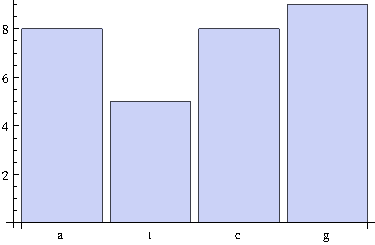
\includegraphics[width=0.4\textwidth]{plot1.pdf}}
  \subfloat{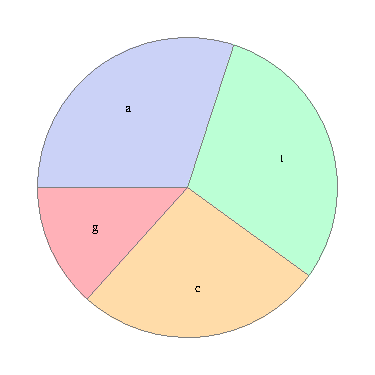
\includegraphics[width=0.4\textwidth]{plot2.pdf}}
\end{figure}

We first generate 2 strings of RNA and convert this to DNA by transforming $u$ to $t$, we then count the number of bases in each string and report this for the first string in a \texttt{BarChart} and for the second string in a \texttt{PieChart}. We then generate the complement strings and show the DNA strings in a \texttt{GridBox}. Lastly we transform this sequence into amino acids, the amino acids are:

Leucine (2x), Valine, Arginine, Proline, Serine, Leucine, Threonine, Proline, Isoleucine.

Leucine, Glycine, Serine, Histidine, Leucine, Methionine, Arginine, Glycine, Asparagine, Threonine.

\subsection{Exercise 3: GenBank Data Files}

In this exercise we use the GenBank file for the Saccharomyces cerevisiae TCP1-beta gene:

\begin{lstlisting}[mathescape]
(*Module to extract the DNA string for a GenBank file*)
Module[{myGenBankfile,OriginRowNumber,DNAsequence,s,proteinseqString,proteinSeqStart,proteinSeqEnd,proteinSeq},
myGenBankfile=ReadList["/home/jhofman/Desktop/CompBio/lab2/U49845.txt",Word, WordSeparators->{"\r"}];
OriginRowNumber=First[Flatten[Position[myGenBankfile,x_String/;x==First[Select[myGenBankfile,StringMatchQ[#,"ORIGIN*"]&]]]]];
DNAseqence=Table[myGenBankfile[[i]],{i,OriginRowNumber+1,Length[myGenBankfile]}];
For[DNAseqString="";i=1,i<Length[DNAseqence]+1,s=StringToStream[DNAseqence[[i]]];DNAseqString=DNAseqString<>StringJoin[Drop[ReadList[s,Word,RecordSeparators->{" "}],1]];i++];
DNAseqString];

(*Count the number of bases and plot the data*)
numOfOcc[sequence_String,base_String]:=Length[Select[Characters[sequence],(#==base)&]];
BarChart[Map[numOfOcc[DNAseqString,#]&,{"a","t","c","g"}],ChartLabels->{"a","t","c","g"}];
PieChart[Map[numOfOcc[DNAseqString,#]&,{"a","t","c","g"}],ChartLabels->{"a","t","c","g"}];

(*Find the string ctcc and number of occurences and highlight them*)
StringPosition[DNAseqString,"ctcc"]
Length[StringPosition[DNAseqString,"ctcc"]]
StringReplace[DNAseqString,x:("ctcc"):>"\!\(\*StyleBox[\""<>x<>"\",FontColor->RGBColor[1,0,0],FontSize->18,FontWeight->\"Bold\"]\)"]
\end{lstlisting}
\begin{lstlisting}[mathescape]
24 
 (5,8),(23,26),(454,457),(470,473),(489,492),(735,738),(1333,1336),(1573,1576),(1643,1646),(1718,1721),(1784,1787),(2066,2069),(2123,2126),(2146,2149),(2602,2605),(2860,2863),(2965,2968),(3350,3353),(3540,3543),(3556,3559),(3651,3654),(4488,4491),(4863,4866),(4965,4968)
\end{lstlisting}

\begin{figure}[H]
  \centering
  \subfloat{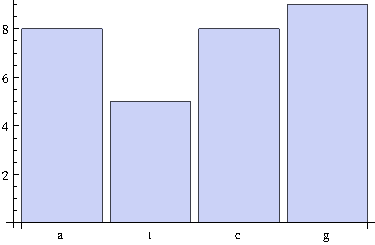
\includegraphics[width=0.4\textwidth]{plot1.pdf}}
  \subfloat{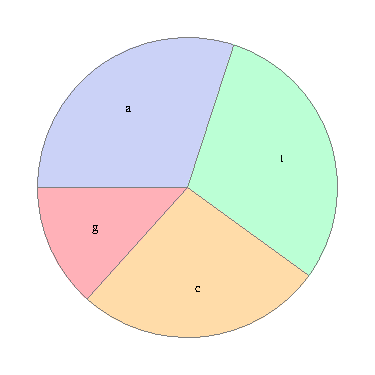
\includegraphics[width=0.4\textwidth]{plot2.pdf}}
\end{figure}

With the above module we can read in the gene sequence (which is large, so we are not going to show it), we then count the number of occurences for each base and plot it in a \texttt{BarChart} and a \texttt{PieChart}. We then search for the string $ctcc$ and report the positions of this string, and then give the number of occurences. Finally we highlight this string in the color red, also not shown because of the size.

\subsection{Exercise 4: Sickle Cell Anemia}
In the last exercise we look at sickle cell anemia, and look at the specific mutation in the DNA which causes this by looking at the hemoglobin gene. We use a GenBank file to read in the hemoglobin gene part of the DNA as well as the specific amino acid sequence. In the following code we omitted the part where the DNA is read in from the file, since it is exactly the same module as in the last exercise. Also we omit the replacement rule which codes triplets of nucleotides to amino acids, also since this is present in the code from the last exercise.

\begin{lstlisting}[mathescape]
(*OMITTED: reading in the file and extracting DNA sequence using the module function of last exercise*)

(*Find position of the nucleotide sequence in which the permutation occurs and apply the permutation*)
position=First[StringPosition[DNAseqString,"ctgactcctgaggagaagtct"]][[1]]
anemia =StringReplace[DNAseqString,"ctgactcctgaggagaagtct"->"ctgactcctgtggagaagtct"]

(*OMITTED: use codon rules to translate triplets to amino acids*)

(*Read in amino acid sequence from file*)
pat2=First[Select[myGenBankfile,StringMatchQ[#,"*translation*"]&]];
pat3=First[Select[myGenBankfile,StringMatchQ[#,"*misc_feature    54..56*"]&]];
proteinSeqStart=First[Flatten[Position[myGenBankfile,x_String/;x==pat2]]];
proteinSeqEnd=First[Flatten[Position[myGenBankfile,x_String/;x==pat3]]]-1;
proteinSeq=Table[myGenBankfile[[i]],{i,proteinSeqStart,proteinSeqEnd}];
StringReplace[StringJoin[proteinSeq],{"\""->""," "->"","/translation="->""}]
\end{lstlisting}

\begin{lstlisting}[mathescape] 
acatttgcttctgacacaactgtgttcactagcaacctcaaacagacaccatggtgcatctgactcctgaggagaag
tctgccgttactgccctgtggggcaaggtgaacgtggatgaagttggtggtgaggccctgggcaggctgctggtggt
ctacccttggacccagaggttctttgagtcctttggggatctgtccactcctgatgctgttatgggcaaccctaagg
tgaaggctcatggcaagaaagtgctcggtgcctttagtgatggcctggctcacctggacaacctcaagggcaccttt
gccacactgagtgagctgcactgtgacaagctgcacgtggatcctgagaacttcaggctcctgggcaacgtgctggt
ctgtgtgctggcccatcactttggcaaagaattcaccccaccagtgcaggctgcctatcagaaagtggtggctggtg
tggctaatgccctggcccacaagtatcactaagctcgctttcttgctgtccaatttctattaaaggttcctttgttc
cctaagtccaactactaaactgggggatattatgaagggccttgagcatctggattctgcctaataaaaaacattta
ttttcattgc

60
acatttgcttctgacacaactgtgttcactagcaacctcaaacagacaccatggtgcatctgactcctgtggagaag
tctgccgttactgccctgtggggcaaggtgaacgtggatgaagttggtggtgaggccctgggcaggctgctggtggt
ctacccttggacccagaggttctttgagtcctttggggatctgtccactcctgatgctgttatgggcaaccctaagg
tgaaggctcatggcaagaaagtgctcggtgcctttagtgatggcctggctcacctggacaacctcaagggcaccttt
gccacactgagtgagctgcactgtgacaagctgcacgtggatcctgagaacttcaggctcctgggcaacgtgctggt
ctgtgtgctggcccatcactttggcaaagaattcaccccaccagtgcaggctgcctatcagaaagtggtggctggtg
tggctaatgccctggcccacaagtatcactaagctcgctttcttgctgtccaatttctattaaaggttcctttgttc
cctaagtccaactactaaactgggggatattatgaagggccttgagcatctggattctgcctaataaaaaacattta
ttttcattgc

TFASDTTVFTSNLKQTPWCI_LLRRSLPLLPCGAR_TWMKLVVRPWAGCWWSTLGPRGSLSPLGICPLLMLLWATLR
_RLMARKCSVPLVMAWLTWTTSRAPLPH_VSCTVTSCTWILRTSGSWATCWSVCWPITLAKNSPHQCRLPIRKWWLV
WLMPWPTSITKLAFLLSNFY_RFLCSLSPTTKLGDIMKGLEHLDSA__KTFIFI

MVHLTPEEKSAVTALWGKVNVDEVGGEALGRLLVVYPWTQRFFESFGDLSTPDAVMGNPKVKAHGKKVLGAFSDGLA
HLDNLKGTFATLSELHCDKLHVDPENFRLLGNVLVCVLAHHFGKEFTPPVQAAYQKVVAGVANALAHKYH
\end{lstlisting}

The above output shows the code extracted from the GenBank file, then finds the pattern and reports its position (60), followed by the DNA code with the mutation (which is labeled red, which is not visible due to \texttt{lstlisting}). Finally we extract the amino acid sequence from this and compare it with the amino acid sequence extracted from the GenBank file. 

There is a very large difference between the two amino acids sequences. The translation provided by the GenBank file is much shorter and contains another sequence. 
This is caused because the translation as provided by the GenBank leaves out all the non-coding parts of the DNA. The coding parts of the DNA start with an $M$, as can also be seen from the translation provided by GenBank. Also the amino acid sequences coding for proteins cannot be really small, i.e. less than 20 amino acids, so also these regions are left out (even though they can start with an $M$) because they cannot code for a protein.

\newpage

\section{Lab3: Enzyme Kinetics }
\subsection{Exercise 1: Ionic Channel Kinetics}

Given the equations:

\begin{align*}
  \frac{dx}{dt} = -k_1 x + k_3 y \nonumber \\
  \frac{dy}{dt} = k_1 x - (k_2 + k_3) y \nonumber \\
  \frac{dz}{dt} = k_2 y
\end{align*}

we can sketch the flow in the (x,y) and the (y,z) plane using the code below, giving the following figures:

\begin{lstlisting}[mathescape]
(* Plot flows at z=0 (first) and x=0 (second) *)
VectorPlot[{-2x+y,2x-3y},{x,0,1},{y,0,1}];
VectorPlot[{2 0-3y,2y},{y,0,1},{z,0,1}];
\end{lstlisting}

\begin{figure}[H]
  \centering
  \subfloat{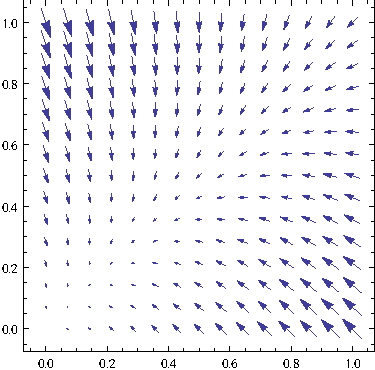
\includegraphics[width=0.4\textwidth]{plot3_1.pdf}}
  \subfloat{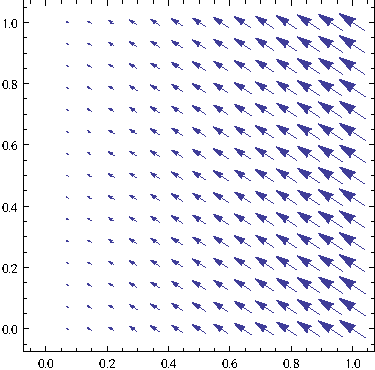
\includegraphics[width=0.4\textwidth]{plot3_2.pdf}}
\end{figure}

We can solve this system numerically ($k_1 = 2, k_2 = 2, k_3 = 1$) by using \texttt{NDSolve} for the initial conditions $x(0) = 1, y(0) = 0$ and $z(0) = 0$. We can do the same for the initial conditions $x(0) = 0, y(0) = 1$ and $z(0) = 0$. The code as well as the figures are given below, the blue line represents $x(t)$, the purple line $y(t)$ and the yellow line $z(t)$:

\begin{lstlisting}[mathescape]
(* Solve and plot with given initial conditions, x=blue, y=purple, z=yellow *)
sol1=NDSolve[{x'[t]== -2x[t]+ y[t],y'[t]==2x[t]-3y[t],z'[t]==2y[t],z[0]==0,x[0]==1,y[0]==0},{x,y,z},{t,0,10}];
Plot[{Evaluate[x[t]/.sol1],Evaluate[y[t]/.sol1],Evaluate[z[t]/.sol1]},{t,0,10},PlotRange->All]
sol2=NDSolve[{x'[t]== -2x[t]+ y[t],y'[t]==2x[t]-3y[t],z'[t]==2y[t],z[0]==0,x[0]==0,y[0]==1},{x,y,z},{t,0,10}];
Plot[{Evaluate[x[t]/.sol2],Evaluate[y[t]/.sol2],Evaluate[z[t]/.sol2]},{t,0,10},PlotRange->All]
\end{lstlisting}

\begin{figure}[H]
  \centering
  \subfloat{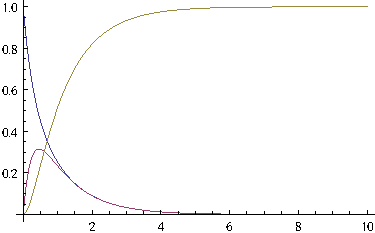
\includegraphics[width=0.4\textwidth]{plot3_3.pdf}}
  \subfloat{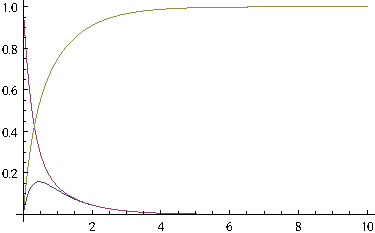
\includegraphics[width=0.4\textwidth]{plot3_4.pdf}}
\end{figure}

As seen in the figures in both cases the quantity of $z$ goes to 1 as $t$ increases. This is logical since the system is only coupled from $y$ to $z$, not the other way around, hence there are fluctuating quantities of $x$ and $y$, but some of the $y$ is depleted and turned into $z$, which then cannot transform into anything else anymore. Hence all the $y$ will slowly change into $z$, and because of this decreasing $y$, more $x$ will be converted to $y$, until everything is converted to $y$, and hence in extension to $z$.

If we change the reaction constants to $k_1 = 0, k_2 = 2$ and $k_3 = 1$ we find the following:

\begin{lstlisting}[mathescape]
(* Changed reaction constants, x=blue, y=purple, z=yellow *)
sol3=NDSolve[{x'[t]== -0x[t]+ y[t],y'[t]==0x[t]-3y[t],z'[t]==2y[t],z[0]==0,x[0]==0,y[0]==1},{x,y,z},{t,0,10}];
Plot[{Evaluate[x[t]/.sol3],Evaluate[y[t]/.sol3],Evaluate[z[t]/.sol3]},{t,0,10},PlotRange->All]
\end{lstlisting}

\begin{figure}[H]
  \centering
  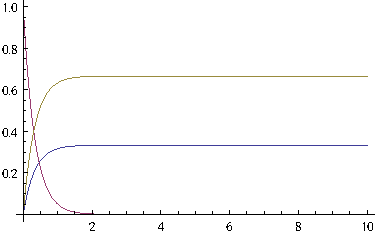
\includegraphics[width=0.4\textwidth]{plot3_5.pdf}
\end{figure}

In this system $z$ does not increase to 1, but an equilibrium is reached in which $y$ is depleted and $x$ and $z$ have some constant nonzero value. Because $k_1 = 0$ there is only a flow away from $y$ to $x$ and $z$ ($\sfrac{dy}{dt} < 0$) and since $y$ connects these two both will end up with some nonzero quantity and equilibrium is reached when $y$ has depleted fully.

If we take $k_1 = 0$ but $k_2$ and $k_3$ arbitrary we can solve the system:

\begin{lstlisting}[mathescape]
(* Exactly solve the system *)
sol4=DSolve[{x'[t]== -0x[t]+ k3 y[t],y'[t]==0x[t]-(k2 + k3)y[t],z'[t]==k2 y[t],z[0]==0,x[0]==0,y[0]==1},{x,y,z},t]
\end{lstlisting}

\begin{lstlisting}[mathescape]
{{x->Function[{t},-(((-1+E^((-k2-k3) t)) k3)/(k2+k3))],y->Function[{t},E^((-k2-k3) t)],z->Function[{t},-(((-1+E^((-k2-k3) t)) k2)/(k2+k3))]}}
\end{lstlisting}

Using the same values of $k$ we can rewrite the system a bit, namely by first differentiating $\sfrac{dy}{dt}$ with respect to $t$ and substituting the expression $\sfrac{dy}{dt}$, which is now on the right hand side, by $k_1 x - (k_2 + k_3) y$, we then obtain:

\begin{align*}
  \frac{d^2 y}{dt^2} &= -k_1^2 x + k_1 k_3 y - k_2 k_1 x - k_3 k_1 x + (k_2 + k_3)^2 y \nonumber \\
  &= (k_2 + k_3)^2 y
\end{align*}

since $k_1 = 0$. With the initial conditions $x(0) = 0, y(0) = 1$ and $z(0) = 0$ we can then obtain the initial conditions:

\begin{align*}
  y[0] = 1 \nonumber \\
  y'[0] = - (k_2 + k_3) y[0] = - (k_2 + k_3) \nonumber \\
  y''[0] = (k_2 + k_3)^2 y[0] = (k_2 + k_3)^2
\end{align*}

Solving this system gives:

\begin{lstlisting}[mathescape]
(* Solving exactly with initial conditions *)
sol5=DSolve[{y''[t] == (k2 + k3)^2y[t],y[0]==1,y'[0]==-(k2+k3),y''[0]==(k2+k3)^2},{y},t] 
\end{lstlisting}

\begin{lstlisting}[mathescape]
{{y->Function[{t},E^((-k2-k3) t)]}}
\end{lstlisting}

which is the same as we obtained in the general case before.

\subsection{Exercise 2: Enzyme inhibition kinetics}
We plot the reaction velocity $V$ as a function of substrate concentration $S$ for a Michaelis-Menten enzyme catalyzed reaction for three different types of inhibitors:

\begin{itemize}
\item 
  competitive: the inhibitor competes with the substrate for binding with the enzyme.
\item
  uncompetitive: the inhibitor binds with the enzyme-substrate product, hence inhibiting the formation of the final product.
\item
  non-competitive: a combination of both, the inhibitor binds with both the substrate as with the enzyme-substrate product.
\end{itemize}

The competitive inhibitor variant can be overcome by increasing the concentration of the substrate since then simply more enzyme-substrate binding will take place. This is however not the case for the uncompetitive variant, since here the intermediate product is involved. Increasing the amount of substrate will also increase the amount of intermediate product but does not affect the amount of this product that binds to the inhibitor, hence the effect of this type of inhibitor is much stronger. Since the non-competitive type has both types incorporated, it has the same effect as the uncompetitive type, which is the stronger one.

We can see this from the figures produced by the code below ($V_{\text{max}} = 1.0, K_M = 1.0, K_i = 1.0, I = 0,2,5,10$), increasing the inhibitor concentration does not decrease the reaction velocity much for the competitive type (left), but it does decrease much for the uncompetitive (middle) and non-competitive types (right).

\begin{lstlisting}[mathescape]
(* Plot reaction velocities with three types of inhibitors *)
Vc[S_,Km_,Ki_,Vmax_,R_]=Vmax S/(S+(1+R/Ki) Km);
Vu[S_,Km_,Ki_,Vmax_,R_]=Vmax S/((1+R/Ki)S+Km);
Vn[S_,Km_,Ki_,Vmax_,R_]=Vmax S/((1+R/Ki)(S+Km));
myplot[A_,i_]:=Plot[A[S,1.0,1.0,1.0,i],{S,0.,200},AxesLabel->{"S ($\mu$M)","Vc ($\mu$M/second)"},PlotRange->All,AxesOrigin->{0,0}]
Show[Table[myplot[Vc,i],{i,{0,2,5,10}}]]
Show[Table[myplot[Vu,i],{i,{0,2,5,10}}]]
Show[Table[myplot[Vn,i],{i,{0,2,5,10}}]] 
\end{lstlisting}

\begin{figure}[H]
  \centering
  \subfloat{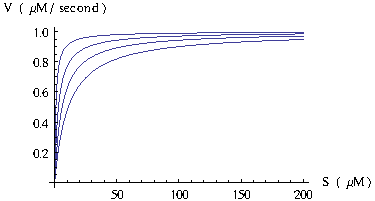
\includegraphics[width=0.33\textwidth]{plot3_6.pdf}}
  \subfloat{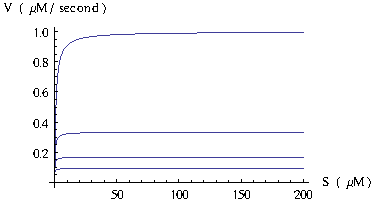
\includegraphics[width=0.33\textwidth]{plot3_7.pdf}}
  \subfloat{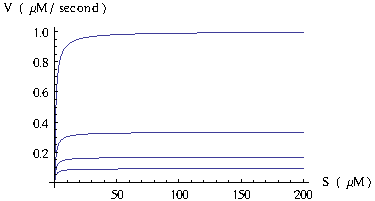
\includegraphics[width=0.33\textwidth]{plot3_8.pdf}}
\end{figure}

\subsection{Exercise 3: Lineweaver-Burke Plot}
We do the same as above, but this time we generate a plot of $\sfrac{1}{V}$ versus $\sfrac{1}{S}$. We first generate a plot without an inhibitor and $K_M = 10, V_{\text{max}} = 25$ and $I = 5,10,15,20$.

\begin{lstlisting}[mathescape]
(* Plot without inhibitor *)
V[S_,Km_,Vmax_]=Vmax (S/(Km+S));
myplot[i_]:=Plot[1/V[1/Sinv,i,25],{Sinv,0,1},AxesLabel->{"S$^{-1}$ (\mu M$^{-1}$)","V$^{-1}$ (\mu M$^{-1}$)"},PlotRange->All,AxesOrigin->{0,0}]
Show[Table[myplot[i],{i,5,20,5}]]
\end{lstlisting}

\begin{figure}[H]
  \centering
  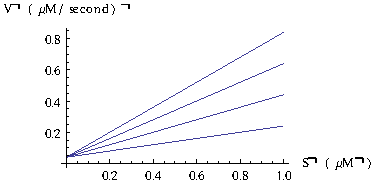
\includegraphics[width=0.4\textwidth]{plot3_9.pdf}
\end{figure}

We then generate a plot for the 3 different types of inhibitors defined above, competitive (left), uncompetitive (middle) and non-competitive (right):

\begin{lstlisting}[mathescape]
myplot[A_,i_]:=Plot[1/A[1/Sinv,1.0,1.0,1.0,i],{Sinv,0.,1},AxesLabel->{"S$^{-1}$ (\mu M$^{-1}$)","V$^{-1}$ (\mu M$^{-1}$)''},PlotRange->All,AxesOrigin->{0,0}]
Show[Table[myplot[Vc,i],{i,{0,2,5,10}}]]
Show[Table[myplot[Vu,i],{i,{0,2,5,10}}]]
Show[Table[myplot[Vn,i],{i,{0,2,5,10}}]] 
\end{lstlisting}

\begin{figure}[H]
  \centering
  \subfloat{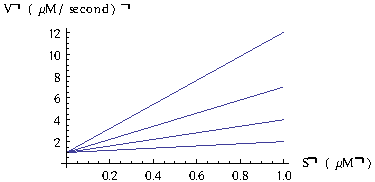
\includegraphics[width=0.4\textwidth]{plot3_10.pdf}}
  \subfloat{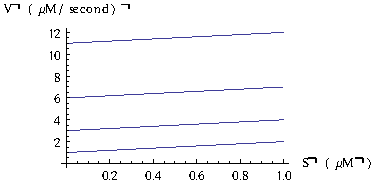
\includegraphics[width=0.4\textwidth]{plot3_11.pdf}}
  \subfloat{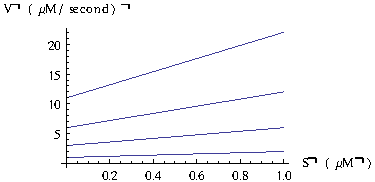
\includegraphics[width=0.4\textwidth]{plot3_12.pdf}}
\end{figure}

Here the difference between competitive and uncompetitive is even more clear than in the last exercise, if all the lines meet around $S^{-1} = 0$ then the reaction velocity is not much affected by changing the inhibitor concentration. In the case of un- or noncompetitive inhibitors however the lines do not meet near zero, indicating that they do not reach the same equilibrium for large concentrations (and hence small $S^{-1}$). Since all the lines get converted to straight lines in the Lineweaver-Burke plots, it is much easier to see whether or not the reaction velocity is affected much by different types of inhibitors.

\subsection{Exercise 4: Derivation of Rate Equations}
On a simple enzyme-substrate reaction of the following form:

\begin{equation*}
  S + E \xleftrightarrow[k2]{k1} SE \xrightarrow{k3} E + P
\end{equation*}

we can apply the law of mass action to obtain the following system of equations:

\begin{align*}
  \frac{d[ES]}{dt} = k_1 [S][E] - k_2 [ES] - k_3 [ES] \nonumber \\
  \frac{d[S]}{dt} = k_2 [ES] - k_1 [E][S] \nonumber \\
  \frac{d[E]}{dt} = k_2 [ES] + k_3 [ES] - k_1 [E][S] \nonumber \\
  \frac{d[P]}{dt} = k_3 [ES]
\end{align*}

If the system is in equilibrium $\frac{d[ES]}{dt} = 0$ and hence $k_1 [S][E] = (k_2 + k_3)[ES]$. If we furthermore assume that the total enzyme concentrations $E_T = [ES] + [E]$ is constant we can combine this to $E_T [S] = (\sfrac{(k_2 + k_3)}{k_1} + [S])[ES]$ and this we can substitute in the expression for $\sfrac{d[P]}{dt}$ to get:

\begin{equation*}
    \frac{d[P]}{dt} = k_3 [ES] = \frac{k_e E_T [S]}{\frac{k_2 + k_3}{k_1} + [S]}
\end{equation*}

which, if we take $k_m = \sfrac{(k_2 + k_3)}{k_1}$ is the correct expression for the reaction rate as a function of substrate concentration $[S]$.

\subsection{Exercise 5: Dependent Gating Channel}
We study a very simple model of gates in the membrane which have the function of transporting ions. The gates are controlled by the membrane potential, described by the mechanism:

\begin{equation*}
  C \xleftrightarrow[k^-]{k^+} O
\end{equation*}

where $C$ is the closed state and $O$ the open state. The fraction of open gates is given by $f_0 = \sfrac{[O]}{([O]+[C])}$ and we can make the following derivation for the derivative of $f_0$ (omitting the $[$ and $]$ from now on):

\begin{align*}
  &\frac{df_0}{dt} = \frac{\sfrac{O}{C+O}}{dt} \nonumber \\
  &= \frac{C+O \frac{dO}{dt} - O \frac{d(C+O)}{dt}}{(C+O)^2} \nonumber \\
  &= \frac{(C+O)(k^+C - k^-O) - 0}{(C+O)^2} \; \text{since C+O is constant} \nonumber \\
  &= \frac{k^+C^2 - k^-OC + k^+OC - k^-O^2}{(C+O)^2} \nonumber \\
  &= k^+(1-f_0)^2 - (k^- - k^+)f_0(1-f_0) - k^-f_o^2 \; \text{since} \; \frac{C}{O+C} = 1 - f_0 \nonumber \\
  &= k^+ - (k^+ + k^-)f_o \nonumber \\
  &= \frac{-(f_0 - f_\infty)}{\tau}  
\end{align*}

if we take $f_{\infty} = \sfrac{k^+}{(k^+ + k^-)}$ and $\tau = \sfrac{1}{(k^+ + k^-)}$. By defining $k^+ = k_0^+ e^{-\alpha V}$ and $k^- = k_0^- e^{-\beta V}$ we can show that (not written out here):

\begin{align*}
  f_\infty = \sfrac{1}{2}(1 + tanh((V-V_0)/2S_0) \\
  \tau = \frac{e^{V(\alpha + \beta)/2}}{2 \sqrt{k_0^+ k_0^-} cosh((V-V_0)/2S_0)}
\end{align*}

where $S_0 = \sfrac{1}{(\beta - \alpha)}$ and $V_0 = \sfrac{ln(k_0^- / k_0^+)}{(\beta - \alpha)}$. Now if we take $\alpha = -\beta$ and define $\phi = \sfrac{1}{2\sqrt{k_0^+ k_0^-}}$ we can plot $f_\infty$ and $\tau$ as a function of the membrane voltage, see the code and figures below. The left figure corresponds to $f_0$ and the right figure corresponds to $\tau$. The red lines have the values $\phi = 5, V_0 = -50$ and $S_0 = -2$, the green line $\phi = 5, V_0 = -25$ and $S_0 = 5$.

\begin{lstlisting}[mathescape]
(* Plot $f_0$ and $\tau$ as a function as a function of $V$ *)
f[V_,V0_,S0_]:=0.5(1+Tanh[(V-V0)/(2S0)]);
$\tau$[V_,V0_,S0_,$\phi$_]:=$\phi$/Cosh[(V-V0)/(2S0)];
Plot[{f[V,-50,-2],f[V,-25,5]},{V,-80,30},PlotRange->All,AxesOrigin->{-80,0},Frame->True,PlotStyle->{Red,Green},FrameLabel->{"V(mV)","f\[Infinity]"},RotateLabel->False]
Plot[{$\tau$[V,-50,-2,5],$\tau$[V,-25,5,5]},{V,-80,30},PlotRange->All,AxesOrigin->{-80,0},Frame->True,PlotStyle->{Red,Green},FrameLabel->{"V(mV)","$\tau$(ms)"},RotateLabel->False]
\end{lstlisting}

\begin{figure}[H]
  \centering
  \subfloat{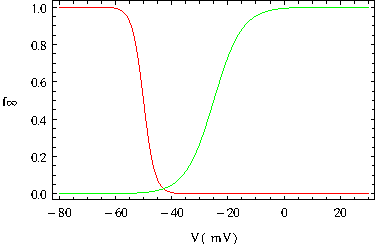
\includegraphics[width=0.4\textwidth]{plot3_13.pdf}}
  \subfloat{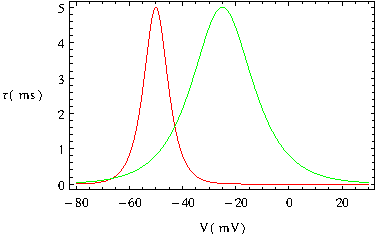
\includegraphics[width=0.4\textwidth]{plot3_14.pdf}}
\end{figure}

The figures represent the figures given in the exercise. If we look at the left figure giving $f_{\infty}$ as a function of $V$ we see that the green line corresponds to an activation channel; as $V$ gets higher the amount of $f_{\infty}$ increases, hence $k_+$ gets dominant and the portion of channels that is open grows. If the voltage is very low $k_+$ is zero and hence all channels will become closed. For the inactivation gate it is the other way around, at low voltages $k_+$ is large and so many channels open, at high voltages they close.

\subsection{Exercise 6: Simple Enzyme Networks}
In this exercise we use the XCellerator package from Mathematica to simulate enzyme networks. We first use the network in Exercise 1, i.e. the ionic channel where $S_1$ is in equilibrium with $S_2$, which can be converted in $S_3$. We can evaluate this system in XCellerator using the following code:

\begin{lstlisting}[mathescape]
(* Reproducing the figures from exercise 1 with XCellerator *)
<< xlr8r.m;
ionicChannel = {
  {A \[RightArrowLeftArrow] B, 2, 1}, {B \[ShortRightArrow] C, 1}
  }
r1 = Quiet[
  run[interpret[ionicChannel], 
   initialConditions -> {A[0] == 1, B[0] == 0, C[0] == 0}, 
   timeSpan -> {0, 10}, plot -> True
   ]]
r2 = Quiet[
  run[interpret[ionicChannel], 
   initialConditions -> {A[0] == 0, B[0] == 1, C[0] == 0}, 
   timeSpan -> {0, 10}, plot -> True
   ]]
\end{lstlisting}

where we first define the system using $A = S_1$, $B = S_2$ and $C = S_3$ and the reaction constants as given in the exercise. We then interpret these equations, which means writing it as a system of coupled ODE's, and next the results are plotted using two types of initial conditions. The results are shown in the two figures below:

\begin{figure}[H]
  \centering
  \subfloat{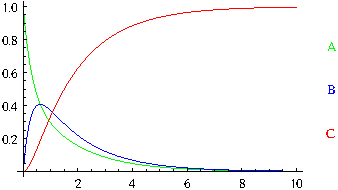
\includegraphics[width=0.4\textwidth]{plot3_15.pdf}}
  \subfloat{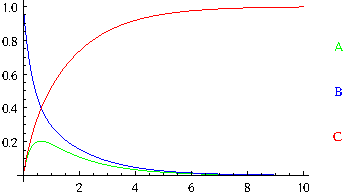
\includegraphics[width=0.4\textwidth]{plot3_16.pdf}}
\end{figure}

where indeed we obtain the same results as in Exercise 1 for the solutions.

We can also use XCellerator to give the system of coupled ODE's. We can do this for the following system:

\begin{align*}
  &S + E \xleftrightarrow[k_1]{k_{-1}} C_1 \xrightarrow[k_2]{} E + P \nonumber \\
  &S + C_1 \xleftrightarrow[k_3]{k_{-3}} C_2 \xrightarrow[k_4]{} C_1 + P \nonumber 
\end{align*}

where we can use the following code to generate the equations:

\begin{lstlisting}[mathescape]
(* Generate allosteric reaction equations *)
allosteric = {
   {S + En \[RightArrowLeftArrow] C1, k1, 
    km1}, {C1 \[ShortRightArrow] En + P, k2},
   {S + C1 \[RightArrowLeftArrow] C2, k3, 
    km3}, {C2 \[ShortRightArrow] C1 + P, k4}
   };
interpret[allosteric]

{{Derivative[1][C1][t] == -k2 C1[t] - km1 C1[t] + k4 C2[t] + 
    km3 C2[t] - k3 C1[t] S[t] + k1 En[t] S[t], 
  Derivative[1][C2][t] == -k4 C2[t] - km3 C2[t] + k3 C1[t] S[t], 
  Derivative[1][En][t] == k2 C1[t] + km1 C1[t] - k1 En[t] S[t], 
  Derivative[1][P][t] == k2 C1[t] + k4 C2[t], 
  Derivative[1][S][t] == 
   km1 C1[t] + km3 C2[t] - k3 C1[t] S[t] - k1 En[t] S[t]}, {C1, C2, 
  En, P, S}}
\end{lstlisting}

where the output gives the system of equations, which can then be solved analytically. Derivative[1][A][B] means $\sfrac{dA}{dB}$ in this case.

\newpage

\section{Lab4: Solving Nonlinear ODE Systems}
\subsection{Exercise 1: Dynamics of Circulating Blood Cells}

We start with a very simple system of ODE's describing the density of circulating blood cells ($x$) controlled by a hormonal agent ($y$):

\begin{align*}
  &\frac{dx}{dt} = \frac{2y}{1 + y^2} - x \nonumber
  &\frac{dy}{dt} = x - y
\end{align*}

We can determine the steady state of this system by solving $\sfrac{dx}{dt} = 0$ and $\sfrac{dy}{dt} = 0$, since in that case the quantities $x$ and $y$ will not change anymore. We can check whether the solution for the steady state is correct by making a plot of the flow of the system. We can also evaluate what happens, given an initial condition, in the limit of $t \rightarrow \infty$.

By solving the system (done by hand) we find $(0,0), (1,1)$ and $(-1,-1)$ as solutions. Since we are interested in the case $x,y \geq 0$ we will discard the last solution. The code below gives a \texttt{streamplot} of the vector field (left figure) where we indeed can see steady states for $(0,0)$ and $(1,1)$. The latter is stable, while the former is not, it is a saddle. We can then solve the system of equations using \texttt{NDSolve} which gives an interpolation of the solution over a certain range, and use that interpolation to plot $x(t)$ versus $y(t)$. with initial conditions $x(0) = 10$ and $y(0) = 0.1$ we see that the solution converges for $t \rightarrow \infty$ to $(1,1)$ (right figure).

\begin{lstlisting}[mathescape]
(* Streamplots and parametric plots of the steady states *)
StreamPlot[{2 y/(1 + y^2) - x, x - y}, {x, -0.5, 2}, {y, -0.5, 2}, 
 ImageSize -> 250]
sol = NDSolve[{x'[t] == (2 y[t]/(1 + y[t]^2) - x[t]), 
    y'[t] == (x[t] - y[t]), x[0] == 10, y[0] == 0.1}, {x, y}, {t, 0, 
    100}];
ParametricPlot[Evaluate[{x[t], y[t]} /. sol], {t, 0, 100}, 
 PlotRange -> All, AxesLabel -> {"x", "y"}, AxesOrigin -> {0, 0}, 
 ImageSize -> 250]
\end{lstlisting}

\begin{figure}[H]
  \centering
  \subfloat{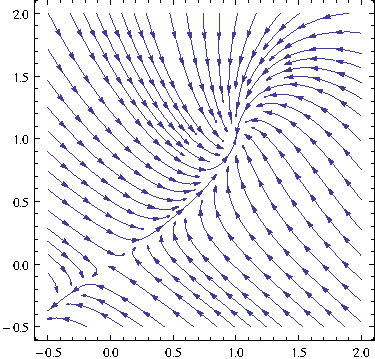
\includegraphics[width=0.4\textwidth]{plot4_1.pdf}}
  \subfloat{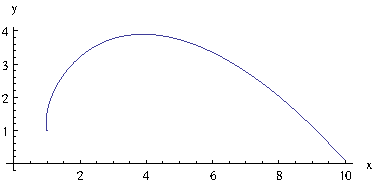
\includegraphics[width=0.4\textwidth]{plot4_2.pdf}}
\end{figure}

\subsection{Exercise 2: Limpets and Seaweed}
We again consider a system of differential equations, this time of limpets ($l$) and seaweed ($s$) which live in a tide pool. The dynamics are described by:

\begin{align*}
  &\frac{ds}{dt} = s - s^2 - sl \nonumber
  &\frac{dl}{dt} = sl - \frac{l}{2} - l^2
\end{align*}

which is a nonlinear system of differential equations making it very hard to solve exactly. We first find the steady states by solving $\frac{ds}{dt} = \frac{dl}{dt} = 0$ and we evaluate the stability by computing the eigenvalues of the Jacobian in the steady states.

\begin{lstlisting}[mathescape]
(* Solve steady state and evaluate stability *)
sol = Solve[{s - s^2 - s l == 0, s l - l/2 - l^2 == 0}, {s, l}]
jac1 = Eigenvalues[
  Outer[D, {s - s^2 - s l, s l - l/2 - l^2}, {s, l}] /. sol[[3]]]
jac1 = Eigenvalues[
  Outer[D, {s - s^2 - s l, s l - l/2 - l^2}, {s, l}] /. sol[[4]]]
\end{lstlisting}

\begin{lstlisting}[mathescape]
{{s -> 0, l -> -(1/2)}, {s -> 0, l -> 0}, {s -> 3/4, 
  l -> 1/4}, {s -> 1, l -> 0}}

{1/4 (-2 + I Sqrt[2]), 1/4 (-2 - I Sqrt[2])}

{-1, 1/2}
\end{lstlisting}

We find four steady states, of which three are nonzero and one does not satisfy the requirement $l,s \geq 0$. The steady state at $(0,0)$ is not interesting because the populations of both species is 0 and the system does not change in time. For the steady state $(\sfrac{3}{4},\sfrac{1}{4})$ we find eigenvalues which have are complex and have negative real part, indicating a stable focus. For the steady state at $(1,0)$ we find real eigenvalues with opposite signs, indicating a saddle point.

We can check whether our stability analysis is correct by making a plot of the flow, given below:

\begin{figure}[H]
  \centering
  \subfloat{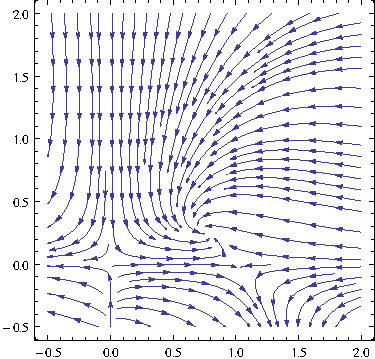
\includegraphics[width=0.4\textwidth]{plot4_3.pdf}}
\end{figure}

As we can see from the figure, there is indeed a stable focus at $(\sfrac{3}{4},\sfrac{1}{4})$ and a saddle at $(1,0)$. We can check the dynamics in the limit of $t \rightarrow \infty$ for the initial conditions by numerically solving the equations and evaluating the interpolation at some large time $t$. We do this with the following code:

\begin{lstlisting}[mathescape]
(* Solving the system of ODE's for different initial values *)
sol1 = NDSolve[{s'[t] == s[t] - s[t]^2 - s[t] l[t], 
    Derivative[1][l][t] == s[t] l[t] - l[t]/2 - l[t]^2, s[0] == 0, 
    l[0] == 0}, {s, l}, {t, 0, 60}];
Evaluate[{s[t], l[t]} /. sol1] /. t -> 60
sol1 = NDSolve[{s'[t] == s[t] - s[t]^2 - s[t] l[t], 
    Derivative[1][l][t] == s[t] l[t] - l[t]/2 - l[t]^2, s[0] == 0, 
    l[0] == 15}, {s, l}, {t, 0, 60}];
Evaluate[{s[t], l[t]} /. sol1] /. t -> 60
sol1 = NDSolve[{s'[t] == s[t] - s[t]^2 - s[t] l[t], 
    Derivative[1][l][t] == s[t] l[t] - l[t]/2 - l[t]^2, s[0] == 2, 
    l[0] == 0}, {s, l}, {t, 0, 60}];
Evaluate[{s[t], l[t]} /. sol1] /. t -> 60
sol1 = NDSolve[{s'[t] == s[t] - s[t]^2 - s[t] l[t], 
    Derivative[1][l][t] == s[t] l[t] - l[t]/2 - l[t]^2, s[0] == 2, 
    l[0] == 15}, {s, l}, {t, 0, 60}];
Evaluate[{s[t], l[t]} /. sol1] /. t -> 60
\end{lstlisting}

\begin{lstlisting}[mathescape]
{{0., 0.}}

{{0., -8.79636*10^-12}}

{{1., -2.16298*10^-27}}

{{0.75, 0.25}}
\end{lstlisting}

Where we find that with initial conditions $(0,0)$, the system stays in $(0,0)$, which is logical since this is a steady state. Furthermore we find that for initial condition $(0,15)$, the system also ends up in $(0,0)$ (indicating that limpets cannot survive without seaweed). For $(2,0)$ we find the system ending up in $(1,0)$ (seaweed can survive without limpets) and for $(2,15)$ finally we find the system ending up in $(\sfrac{3}{4},\sfrac{1}{4})$ (mutual benefit between the species).

\subsection{Exercise 3: Brusselator Oscillator}
We now look at a model for chemical oscillations, the Brusselator, given by:

\begin{align*}
  &\frac{du}{dt} = a - (b + 1)u + u^2 v \nonumber
  &\frac{dv}{dt} = b u - u^2 v
\end{align*}

with $a,b$ positive constants and $u,v \geq 0$. We first determine the steady state in terms of $a$ and $b$ and then find the characteristic equation in terms of $\lambda$ for the eigenvalues of the Jacobian in this steady state and solve this for $\lambda$:

\begin{lstlisting}[mathescape]
(* Find steady state and solve characteristic equation for stability *)
sol = Solve[{a - (b + 1) u + u^2 v == 0, b u - u^2 v == 0}, {u, v}]
eq = Det[(Outer[D, {a - (b + 1) u + u^2 v, b u - u^2 v}, {u, v}] /. 
     Flatten[sol]) - $\lambda$ IdentityMatrix[2]]
Solve[eq == 0, $\lambda$]
\end{lstlisting}

\begin{lstlisting}[mathescape]
{{u -> a, v -> b/a}}

a^2 + $\lambda$ + a^2 $\lambda$ - b $\lambda$ + $\lambda$^2

{{$\lambda$ -> 
   1/2 (-1 - a^2 - Sqrt[-4 a^2 + (1 + a^2 - b)^2] + b)}, {$\lambda$ ->
    1/2 (-1 - a^2 + Sqrt[-4 a^2 + (1 + a^2 - b)^2] + b)}}
\end{lstlisting}

We see that the steady state is given by $(a,\sfrac{b}{a})$ and we find a corresponding characteristic equation for the eigenvalues in this steady state given by $a^2 + \lambda + a^2 \lambda - b \lambda + \lambda^2$. We can then solve this for $\lambda$ where we obtain a general expression for the eigenvalues in terms of $a$ and $b$.

We will check the behavior of $v(t)$ for a constant concentration $u(t) = u(0)$ (assuming $b$ = 1). If we take $u(t) = 5$ and we vary the concentration of $v(0)$ we see that the behavior as $t \rightarrow \infty$ is independent of the initial conditions:

\begin{lstlisting}[mathescape]
(* Solving the system for different initial conditions (b=1) *)
sol1 = Table[
   NDSolve[{u'[t] == 0, v'[t] == (b u[t] - u[t]^2 v[t]) /. b -> 1, 
     v[0] == i, u[0] == 5}, {u, v}, {t, 0, 100}], {i, 0, 4, 2}];
Show[Plot[Evaluate[{v[t]} /. sol1[[1]]], {t, 0, 1}, 
  PlotRange -> {{0, 0.4}, {0, 5}}, AxesLabel -> {"t", "v[t]"}, 
  PlotStyle -> Blue, ImageSize -> 250],
 Plot[Evaluate[{v[t]} /. sol1[[2]]], {t, 0, 1}, 
  PlotRange -> {{0, 0.4}, {0, 5}}, AxesLabel -> {"t", "v[t]"}, 
  PlotStyle -> Red, ImageSize -> 250], 
 Plot[Evaluate[{v[t]} /. sol1[[3]]], {t, 0, 1}, 
  PlotRange -> {{0, 0.4}, {0, 5}}, AxesLabel -> {"t", "v[t]"}, 
  PlotStyle -> Green, ImageSize -> 250]]
\end{lstlisting}

\begin{figure}[H]
  \centering
  \subfloat{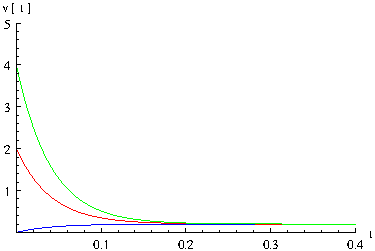
\includegraphics[width=0.4\textwidth]{plot4_4.pdf}}
\end{figure}

Hence given a fixed concentration $u(t)$ the system does not depend on initial concentrations $v(t)$ after some time $t$.

We can find the bifurcation point of this system by checking when the trace of the Jacobian at the steady state changes sign:

\begin{lstlisting}[mathescape]
Tr[Outer[D, {a - (b + 1) u + u^2 v, b u - u^2 v}, {u, v}] /. 
  Flatten[sol]]
\end{lstlisting}
 
\begin{lstlisting}[mathescape]
-1 - a^2 + b
\end{lstlisting}

and we see that his happens (taking $a = 1$) when $b = 2$. We can check this by looking at the behavior of $u,v$ for $b = 1.5$ and $b = 2.5$, see the code and the figure below. We see that for $b = 2.5$ the solution converges to a stable focus. In the case of $b = 1.5$ the solution converges to a limit cycle, given the same initial conditions, so indeed the system behaves differently above and below this bifurcation point.

\begin{lstlisting}[mathescape]
(* Solve around the bifurcation point and plot *)
sol1 = NDSolve[{u'[t] == (a - (b + 1) u[t] + u[t]^2 v[t]) /. {a -> 1, 
      b -> 2.5}, v'[t] == (b u[t] - u[t]^2 v[t]) /. b -> 2.5, 
    v[0] == 0, u[0] == 5}, {u, v}, {t, 0, 100}];
sol2 = NDSolve[{u'[t] == (a - (b + 1) u[t] + u[t]^2 v[t]) /. {a -> 1, 
      b -> 1.5}, v'[t] == (b u[t] - u[t]^2 v[t]) /. b -> 1.5, 
    v[0] == 0, u[0] == 5}, {u, v}, {t, 0, 100}];
Show[ParametricPlot[Evaluate[{u[t], v[t]} /. sol2], {t, 0, 100}, 
  PlotRange -> All, AxesLabel -> {"u[t]", "v[t]"}, PlotStyle -> Blue, 
  ImageSize -> 250], 
 ParametricPlot[Evaluate[{u[t], v[t]} /. sol1], {t, 0, 100}, 
  PlotRange -> All, AxesLabel -> {"u[t]", "v[t]"}, PlotStyle -> Red, 
  ImageSize -> 250]]
\end{lstlisting}

\begin{figure}[H]
  \centering
  \subfloat{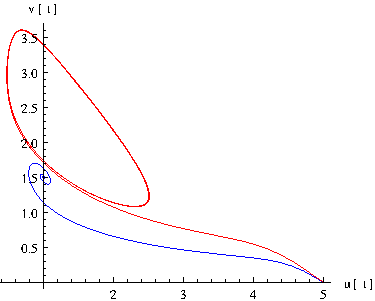
\includegraphics[width=0.4\textwidth]{plot4_5.pdf}}
\end{figure}

\subsection{Exercise 4: Fitzhugh-Nagumo Equations}
In this exercise we look at the Fitzhugh-Nagumo equations, which are used for modeling neuron systems. The dynamics are described by the following equations:

\begin{align*}
  &\frac{dx}{dt} = \frac{1}{\epsilon}(y - \frac{x^3}{12} + x) \nonumber 
  &\frac{dy}{dt} = - \epsilon (2x + y - \frac{8}{3})
\end{align*}

We can, like in the previous exercises, find the steady state and evaluate the stability in this steady state, as shown in the code below. We find a steady state at $(2,\sfrac{-4}{3})$ and 2 other imaginary steady states, which cannot represent a real solution. The eigenvalues of this steady state are complex with negative real part, as $0 < \epsilon \leq 1$, which indicates a stable focus.

\begin{lstlisting}[mathescape]
(* Stability analysis of the system and interpolation plots for different initial values *)
sol = Solve[{1/$\epsilon$ (y - x^3/12 + x) == 
    0, -$\epsilon$ (2 x + y - 8/3) == 0}, {x, y}]
jac1 = Eigenvalues[
  Outer[D, {1/$\epsilon$ (y - x^3/12 + x), -$\epsilon$ (2 x + y - 
        8/3)}, {x, y}] /. sol[[1]]]

sol1 = NDSolve[{x'[
       t] == (1/$\epsilon$ (y[t] - x[t]^3/12 + x[t])) /. $\epsilon$ ->
       0.1, y'[
       t] == (-$\epsilon$ (2 x[t] + y[t] - 8/3)) /. $\epsilon$ -> 0.1,
     x[0] == 1, y[0] == -4/3}, {x, y}, {t, 0, 100}];
sol2 = NDSolve[{x'[
       t] == (1/$\epsilon$ (y[t] - x[t]^3/12 + x[t])) /. $\epsilon$ ->
       0.1, y'[
       t] == (-$\epsilon$ (2 x[t] + y[t] - 8/3)) /. $\epsilon$ -> 0.1,
     x[0] == -4, y[0] == 4}, {x, y}, {t, 0, 100}];
sol3 = NDSolve[{x'[
       t] == (1/$\epsilon$ (y[t] - x[t]^3/12 + x[t])) /. $\epsilon$ ->
       0.1, y'[
       t] == (-$\epsilon$ (2 x[t] + y[t] - 8/3)) /. $\epsilon$ -> 0.1,
     x[0] == 2, y[0] == -4}, {x, y}, {t, 0, 100}];
Show[StreamPlot[{(1/$\epsilon$ (y - x^3/12 + x)) /. $\epsilon$ -> 
     0.1, (-$\epsilon$ (2 x + y - 8/3)) /. $\epsilon$ -> 0.1}, {x, -5,
    5}, {y, -5, 5}],
ParametricPlot[Evaluate[{x[t], y[t]} /. sol1], {t, 0, 100}, 
  PlotRange -> All, AxesLabel -> {"x", "y"}, AxesOrigin -> {0, 0}, 
  PlotStyle -> Red],
ParametricPlot[Evaluate[{x[t], y[t]} /. sol2], {t, 0, 100}, 
  PlotRange -> All, AxesLabel -> {"x", "y"}, AxesOrigin -> {0, 0}, 
  PlotStyle -> Blue], 
ParametricPlot[Evaluate[{x[t], y[t]} /. sol3], {t, 0, 100}, 
  PlotRange -> All, AxesLabel -> {"x", "y"}, AxesOrigin -> {0, 0}, 
  PlotStyle -> Green], ImageSize -> 250]
\end{lstlisting}

\begin{lstlisting}[mathescape]
{{x -> 2, y -> -(4/3)}, {x -> -1 - I Sqrt[15], 
  y -> 2/3 (7 + 3 I Sqrt[15])}, {x -> -1 + I Sqrt[15], 
  y -> 2/3 (7 - 3 I Sqrt[15])}}

{1/2 (-$\epsilon$ - Sqrt[-8 + $\epsilon$^2]), 
 1/2 (-$\epsilon$ + Sqrt[-8 + $\epsilon$^2])} 
\end{lstlisting}

Assuming $\epsilon = 0.1$, we can solve the system of equations, using various initial conditions, one of which is $x(0) = 1, y(0) = \sfrac{-4}{3}$. The figure below shows the orbit of $(x,y)$ for various initial conditions. Clearly we see from the figure that small deviations from the steady state (i.e. starting in $(1,\sfrac{-4}{3})$) lead to large detours before the system is ending up in the steady state. 

\begin{figure}[H]
  \centering
  \subfloat{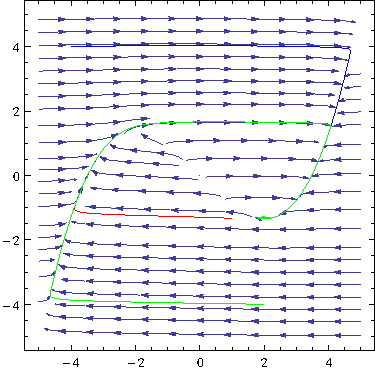
\includegraphics[width=0.4\textwidth]{plot4_6.pdf}}
\end{figure}

\subsection{Exercise 5: Morris-Lecar Model}

In this exercise we study the Morris Lecar model, which describes the reaction of muscle fibers under the injection of a constant current. This model can be described by a system of differential equations:

\begin{align*}
  &C \frac{dV}{dt} = -g_{\text{Ca}} m_{\infty} (V - V_{\text{Ca}}) - g_K w (V - V_K) - g_L (V - V_L) + I_{\text{app}} \nonumber
  &\frac{dw}{dt} = \frac{\phi (w_\infty - w)}{\tau}
\end{align*}

where $m_\infty = 0.5(1 + \text{tanh}((V-v_1)/v_2))$, $w_\infty = 0.5(1 + \text{cosh}((V-v_3)/v_4)$ and $\tau = 1/\text{cosh}((V-v_3)/2v_4)$. If we use the parameters as given in the exercise we can solve this system by interpolation, and plot the concentration $V(t)$, given in the figure below where we see a large fluctuation of $V(t)$ as a function of time. The black line corresponds with $I_{\text{app}} = 60$, the blue line with $I_{\text{app}} = 150$ and the red line for $I_{\text{app}} = 200$. The fluctuation grows with increasing $I_{\text{app}}$ and for low $I_{\text{app}}$ there is only a single excitation without any fluctuating behavior.

\begin{lstlisting}[mathescape]
(* Solve and interpolate the system for different values of I *)
sol = Table[
   NDSolve[{20*
       V'[t] == -4.4*0.5 (1 + Tanh[(V[t] + 1.2)/18]) (V[t] - 120) - 
       8*w[t] (V[t] + 84) - 2 (V[t] + 60) + i, 
     w'[t] == 
      0.04*(0.5 (1 + Tanh[(V[t] - 2)/30]) - w[t])/(1/
          Cosh[(V[t] - 2)/(2*30)]), V[0] == 0, w[0] == 0}, {V, w}, {t,
      0, 200}], {i, {60, 150, 200}}] ;
Plot[{Evaluate[{V[t]} /. sol[[1]]], Evaluate[{V[t]} /. sol[[2]]], 
  Evaluate[{V[t]} /. sol[[3]]]}, {t, 0, 200}, PlotRange -> All, 
 AxesLabel -> {"t", "V[t]"}, PlotStyle -> {Black, Blue, Red}, 
 ImageSize -> 250]
\end{lstlisting}

\begin{figure}[H]
  \centering
  \subfloat{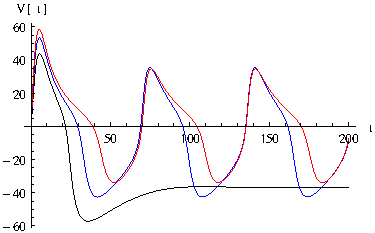
\includegraphics[width=0.4\textwidth]{plot4_7.pdf}}
\end{figure}

We can also plot the orbit $(V,w)$ with initial conditions $V(0) = 0, w(0) = 0$ together with the flow for these three situations, see the figures below for $I_{\text{app}} = 60$ (black), 150 (red) and 200 (blue). It is not that clearly visible in the figure due to weird plotting, but the black line indeed ends in a steady state, whereas the red and blue lines keep oscillating. 

\begin{lstlisting}
(* Plot for different values of $I$, with the same initial condition *)
Show[VectorPlot[{-4.4*0.5 (1 + Tanh[(V + 1.2)/18]) (V - 120) - 
    8*w (V + 84) - 2 (V + 60) + 150, 
   0.04*(0.5 (1 + Tanh[(V - 2)/30]) - w)/(1/
       Cosh[(V - 2)/(2*30)])}, {V, -50, 50}, {w, -1, 1}],
ParametricPlot[{Evaluate[{V[t], w[t]} /. sol[[1]]], 
   Evaluate[{V[t], w[t]} /. sol[[2]]], 
   Evaluate[{V[t], w[t]} /. sol[[3]]]}, {t, 0, 200}, 
  AxesLabel -> {"V", "w"}, PlotStyle -> {Black, Blue, Red}]]  
\end{lstlisting}

\begin{figure}[H]
  \centering
  \subfloat{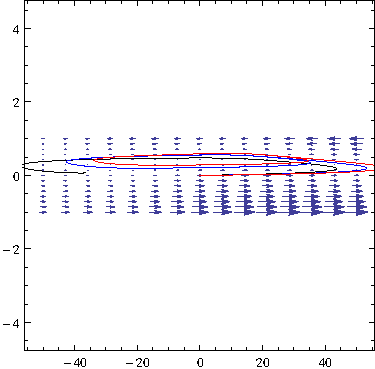
\includegraphics[width=0.4\textwidth]{plot4_8.pdf}}
\end{figure}

\newpage

\section{Lab5: Compartmental Modeling}
\subsection{Exercise 1: Limit Cycle and Chaotic Behavior}
In this exercise we use the code provided in the Notebook and alter the parameter $Kcm$ to show that there exists solutions which are 2-fold limit cycles or chaotic behavior. The code is given below, as well as the behavior:

\begin{lstlisting}[mathescape]
Clear[t, x, y, z]; Kch = 4000;
solution = 
 NDSolve[{Derivative[1][x][t] == 
    Kch (x[t]^2 (y[t] - x[t]))/(25 + x[t]^2) + 0.05 (y[t] - x[t]) - 
     20 x[t] + (125 x[t]^2/(x[t]^2 + 25) + 0.00625) z[t] - 
     300 x[t]^ 8/(0.8^ 8 + x[t]^ 8) + 
     0.01 (90 - x[t] - 4 y[t] - 4 z[t]) - 
     0.1 x[t] (30 + x[t] + 4 y[t] + 4 z[t]), 
   Derivative[1][y][
     t] == - (1/
      4) (Kch (x[t]^2 (y[t] - x[t]))/(25 + x[t]^2) + 
       0.05 (y[t] - x[t]) - 20 x[t]), 
   Derivative[1][z][
     t] == - (1/
      4) ((125 x[t]^2/(x[t]^2 + 25) + 0.00625) z[t] - 
       300 x[t]^ 8/(0.8^ 8 + x[t]^ 8)), x[0] == 0.3, y[0] == 0.2, 
   z[0] == 1.0}, {x, y, z}, {t, 0, 300}, 
  MaxSteps -> 30000]; ParametricPlot[
 Evaluate[{z[t], x[t]} /. solution], {t, 100, 200}, 
 PlotPoints -> 3000, PlotRange -> All]
\end{lstlisting}

\begin{figure}[H]
  \centering
  \subfloat{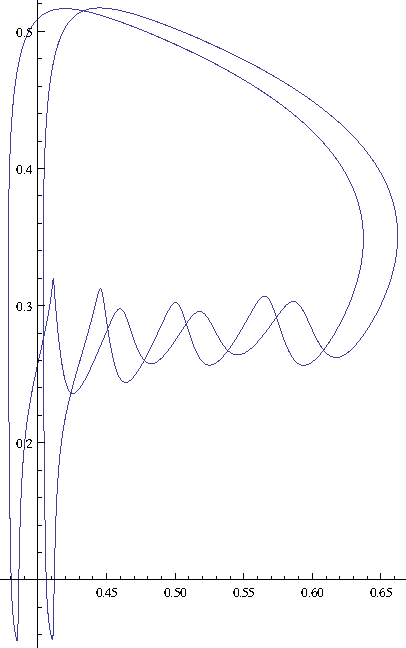
\includegraphics[width=0.4\textwidth]{plot5_1.pdf}}
  \subfloat{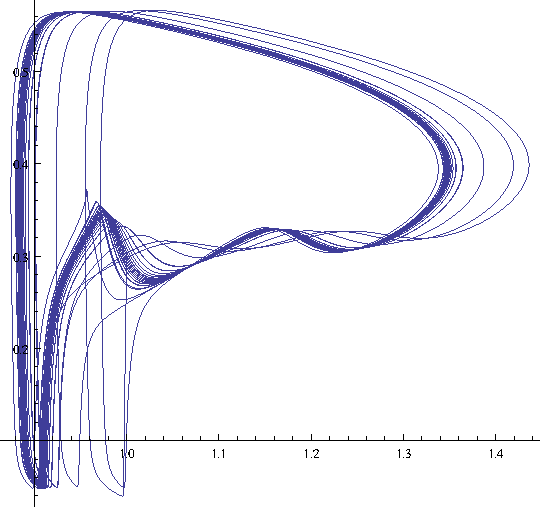
\includegraphics[width=0.4\textwidth]{plot5_2.pdf}}
\end{figure}

The code for the second figure is not given, since that is just a matter of changing the parameter $Kcm$. Clearly we see a two-folded limit cycle ($Kcm$ = 4000) as well as chaotic behavior in the second picture ($Kcm$ = 2950), the values are obtained from the paper mentioned in the exercise.

\subsection{Exercise 2: Slight Model Modifications}

We have the system of equations describing calcium concentrations in the endoplasmatic reticulum (ER), cytosol (cyt) and mitochondria (m) given by:

\begin{align*}
  &\frac{dCa_{\text{cyt}}}{dt} = J_{\text{ch}} + J_{\text{leak}} - J_{\text{pum}} + J_{\text{out}} - J_{\text{in}} + k_-CaPr - k_+Ca_{\text{cyt}}Pr \nonumber \\
  &\frac{dCa_{\text{ER}}}{dt} = \frac{\beta_{\text{ER}}}{\rho_{\text{ER}}}(J_{\text{pump}} - J_{\text{ch}} + J_{\text{leak}}) \nonumber \\
  &\frac{dCa_{\text{m}}}{dt} = \frac{\beta_{\text{m}}}{\rho_{\text{m}}}(J_{\text{in}} - J_{\text{out}})
\end{align*}

We assume now that the channel protein which transports the calcium ions from the ER into the cytosol does not exist anymore, the equations can then be rewritten to:

\begin{align*}
  &\frac{dCa_{\text{cyt}}}{dt} = J_{\text{leak}} - J_{\text{pump}} + J_{\text{out}} - J_{\text{in}} + k_-CaPr - k_+Ca_{\text{cyt}}Pr \nonumber \\
  &\frac{dCa_{\text{ER}}}{dt} = \frac{\beta_{\text{ER}}}{\rho_{\text{ER}}}(J_{\text{pump}} + J_{\text{leak}}) \nonumber \\
  &\frac{dCa_{\text{m}}}{dt} = \frac{\beta_{\text{m}}}{\rho_{\text{m}}}(J_{\text{in}} - J_{\text{out}})
\end{align*}

i.e. leaving out $J_{\text{ch}}$. Another possibility is involving the Golgi complex which has a pump for calcium from the cytosol into the complex ($J_{\text{gpump}}$) and a leak flux into the cytosol ($J_{\text{gleak}}$), the equations will then become:

\begin{align*}
  &\frac{dCa_{\text{cyt}}}{dt} = J_{\text{ch}} + J_{\text{leak}} + J_{\text{gleak}} - J_{\text{gpump}} - J_{\text{pump}} + J_{\text{out}} - J_{\text{in}} + k_-CaPr - k_+Ca_{\text{cyt}}Pr \nonumber \\
  &\frac{dCa_{\text{ER}}}{dt} = \frac{\beta_{\text{ER}}}{\rho_{\text{ER}}}(J_{\text{pump}} - J_{\text{ch}} + J_{\text{leak}}) \nonumber \\
  &\frac{dCa_{\text{m}}}{dt} = \frac{\beta_{\text{m}}}{\rho_{\text{m}}}(J_{\text{in}} - J_{\text{out}}) \nonumber \\
  &\frac{dCa_{\text{golgi}}}{dt} = J_{\text{gpump}} - J_{\text{gleak}}
\end{align*}

\end{document}
